%
% main.tex -- Paper zum Thema <julia>
%
% (c) 2020 Autor, OST Ostschweizer Fachhochschule
%
% !TEX root = ../../buch.tex
% !TEX encoding = UTF-8
%
\chapter{Julia-Mengen und Mandelbrot-Menge\label{chapter:julia}}
\kopflinks{Julia-Mengen und Mandelbrot-Menge}
\begin{refsection}
\chapterauthor{Nicola Dall'Acqua}

Julia-Mengen und die Mandelbrot-Menge entstehen, wenn Kompositionen von holomorphen Funktionen mit sich selbst betrachtet werden.
Konkret wird untersucht, wie sich Funktionen verhalten, wenn diese iteriert auf sich selbst angewendet werden.
Dieses Gebiet wird auch als \emph{komplexe Dynamik} oder \emph{holomorphe Dynamik} bezeichnet.

Das Interesse an dieser Idee lässt sich beispielsweise mit numerischen Methoden, wie dem Newton-Algorithmus motivieren.
Dieser kann zur Lösung der Gleichung
\begin{equation*}
    x^2 + a = 0
    \label{beispielgleichung}
\end{equation*}
herangezogen werden.

Die Iterationsformel lautet
\begin{equation*}
    x_{n + 1} = x_n - \frac{f(x_n)}{f^\prime(x_n)} = x_n - \frac{x_n^2 + a}{2x_n}.
\end{equation*}
Was sich hinter dieser Formel verbirgt, ist nichts weiter als eine Komposition von einer Funktion $f$ mit sich selbst --- man erhält den nächsten Wert $x_{n + 1}$, indem man die Funktion $f$ auf den aktuellen Wert $x_n$ anwendet.

Die Gleichung \eqref{beispielgleichung} besitzt einen Parameter $a$, ist $a = 1$, so erreicht der Newton-Algorithmus keine Konvergenz in den reellen Zahlen.
Weiter kann der Algorithmus ein schlechtes Resultat liefern, wenn der Startwert $x_0$ weit weg von der exakten Lösung gewählt wird.
Die Iteration der Funktion $f$ kann sich also, basierend auf verschiedenen Umständen, auf verschiedene Weisen verhalten.

Für das genaue Verständnis der Folge $x_0,\, x_1,\, x_2,\, \ldots$, welche durch die Iteration von $f$ entsteht, müssen also Hilfsmittel entwickelt werden.
Dies führt schlussendlich zu den Julia-Mengen --- und den Fatou-Mengen, welche das Komplement der Julia-Mengen sind --- sowie der Mandelbrot-Menge.

\section{Julia-Mengen und Fatou-Mengen}
\label{sec:julia}
Julia-Mengen und Fatou-Mengen entstehen aus der Überlegung was geschieht, wenn man eine Funktion $f$ wiederholt auf ein $z \in \mathbb{C}$ anwendet.
Hierraus ergibt sich für jedes $z$ eine Folge komplexer Zahlen
\begin{equation}
    z \rightarrow f(z) \rightarrow f(f(z)) \rightarrow \ldots \:,
    \label{julia_folge}
\end{equation}
bzw.
\begin{equation*}
    z_{n + 1} = f(z_n) \quad \text{mit}\: n \in \mathbb{N}_0\: \text{und einem Startwert}\: z_0 \in \overline{\mathbb{C}} = \mathbb{C} \cup \infty.
\end{equation*}

Je nach Wahl des Startwerts $z_0$ kann diese Folge zwei Verhalten zeigen:
\begin{enumerate}
    \item Eine kleine Änderung des Startwerts führt zur praktisch derselben Folge. Der Wert $z_0$ wird der Fatou-Menge $F_f$ von $f$ zugeordnet.
    \item Eine kleine Änderung des Startwerts führt zu einer komplett anderen Folge. In diesem Fall wird $z_0$ der Julia-Menge $J_f$ von $f$ zugeordnet.
\end{enumerate}

\subsection{Periodische Folgen}
Das Verhalten von solchen Folgen ist besonders dann interessant, wenn diese periodisch sind, bzw. $z_n = z_0$ für ein $n > 0$ gilt.
In dem Fall wird $z_0$ als \emph{periodischer Punkt} bezeichnet.
Ist $n$ die kleinste natürliche Zahl mit dieser Eigenschaft, so heisst $n$ die \emph{Periode} des Zyklus.
Falls dies bereits für $n = 1$ zutrifft, wenn also $f(z_0) = z_0$ gilt, so ist $z_0$, nicht nur ein periodischer Punkt, sondern auch ein \emph{Fixpunkt} von $f$.
Aus diesen Definitionen geht hervor, dass ein periodischer Punkt von $f$ mit Periode $n$ gleichzeitig ein Fixpunkt der $n$-fach zusammengesetzten Funktion $f^n$ ist.

Um die Komplexität der Fragestellung zu reduzieren, werden zunächst nur Fixpunkte betrachtet.

\subsubsection{Erstes Beispiel}
Am Beispiel der Funktion 
\begin{equation*}
    f(z) = z^2,
\end{equation*}
lassen sich solche periodische Folgen beobachten.
Durch $n$-maliges Anwenden erhält man $f^n(z) = z^{2^n}$.
Weiter hat die Funktion $f$ drei Fixpunkte: $0, 1$ und $\infty$, denn für diese Punkte gilt $f(z_0) = z_0$.

Entwickelt man nun die Folge \eqref{julia_folge}, ausgehend von den Startwerten $0$ und $\infty$, so erhält man $f^n(0) = 0$ bzw. $f^n(\infty) \to \infty$.
Nun werden diese Startwerte leicht verändert, dies geschieht mittels einem $\varepsilon \ll 1$:
\begin{itemize}
    \item Für $z_0 = 0$: $f^n(0 + \varepsilon) = (0 + \varepsilon)^{2^n} \to 0$ mit $|\varepsilon| > 0$
    \item Für $z_0 \to \infty$: $f^n(\infty + \varepsilon) = (\infty + \varepsilon)^{2^n} \to \infty$ mit $|\varepsilon| > 0$
\end{itemize}
Obwohl die Startwerte verändert wurden, erhält man schlussendlich die gleichen Resultate, wie wenn man die Startwerte nicht verändert hätte.
Anders ausgedrückt führen kleine Änderungen der Startwerte zu praktisch denselben Folgen.
Es scheint, dass diese beiden Startwerte Folgen in ihrer Umgebung anziehen.

Für den Startwert $1$ erhält man $f^n(1) = 1$, durch leichtes Verändern jedoch:
\begin{itemize}
    \item $f^n(1 + \varepsilon) = (1 + \varepsilon)^{2^n} \to \infty$ mit $\varepsilon > 0$
    \item $f^n(1 - \varepsilon) = (1 - \varepsilon)^{2^n} \to 0$ mit $\varepsilon > 0$
\end{itemize}
Hier scheint es also, dass eine kleine Änderung des Startwerts zu einer ganz anderen Folge führt, dieser Startwert stösst Folgen in seiner nahen Umgebung weg.

\subsubsection{Zweites Beispiel}
Als zweites Beispiel dient die Funktion
\begin{equation*}
    h(z) = z + z^7.
\end{equation*}
Diese Funktion hat Fixpunkte bei $-\infty, 0$ und $\infty$.
Die Fixpunkte $-\infty$ und $\infty$ verhalten sich erneut anziehend und werden daher nicht näher untersucht.
Nimmt man jedoch $0$ als Startwert, passiert etwas anderes.
Zunächst ergibt sich $h^n(0) = 0$, durch eine kleine Änderung erhält man,
\begin{equation*}
    h(0 + \varepsilon) = (0 + \varepsilon) + (0 + \varepsilon)^7 \text{ mit } 0 < |\varepsilon| \ll 1.
\end{equation*}
Da es sich bei $\varepsilon$ um eine sehr kleine Zahl handelt, verschwindet der zweite Summand und übrig bleibt der lineare Term.
Somit ist
\begin{equation*}
    h(0 + \varepsilon) = 0 + \varepsilon.
\end{equation*}
Wendet man nun erneut $h$ auf dieses Resultat an, erhält man wieder $0 + \varepsilon$.
Auch durch $n$-maliges Anwenden von $h$ ändert sich das Resultat nicht.
Die Folge bewegt sich also, anders als vorhin, nicht.
Der Startwert $0$, scheint also Folgen weder abzustossen, noch anzuziehen.

\subsubsection{Arten von periodischen Punkten}
\label{arten_periodische_punkte}
Das Verhalten einer Folge hängt also von der Art der periodischen Punkte ab.
Sei $z_0$ ein periodischer Punkt von $f$ mit Periode $n$, demzufolge ist $z_0$ ein Fixpunkt von $g = f^n$.
Dadurch wird die Frage nach dem Verhalten in der Nähe eines periodischen Punktes reduziert, auf die Frage nach dem Verhalten in der Nähe eines Fixpunktes.
Diese Frage lässt sich mithilfe der Taylorreihe um $z_0$
\begin{equation*}
    g(z) \approx z_0 + g^\prime(z_0) (z - z_0)
    \label{taylor}
\end{equation*}
beantworten, wobei höhere Potenzen in der Nähe von $z_0$ verschwinden.
Verwendet man $z_0$ als Startwert und ändert diesen leicht, bedeutet dies
\begin{equation*}
    z = z_0 + \varepsilon \text{ mit } |\varepsilon| > 0.
\end{equation*}
Setzt man dies in die Taylorreihe ein, erhält man
\begin{equation*}
    g(z) = g(z_0 + \varepsilon) \approx z_0 + g^\prime(z_0) \left((z_0 + \varepsilon) - z_0\right) = z_0 + g^\prime(z_0) \varepsilon.
\end{equation*}
Wird $g$ erneut und wiederholt auf dieses Resultat angewendet, so wird das Verhalten der entstehenden Folge einzig von $g^\prime(z_0)$ festgelegt.
Ist $|g^\prime(z_0)| < 1$, so wird der zweite Summand durch wiederholte Anwendungen immer kleiner und die Folge kehrt zu $z_0$ zurück.
Bei $|g^\prime(z_0)| = 0$ geschieht dies bereits nach der ersten Anwendung von $g$.
Im Fall dass $|g^\prime(z_0)| > 1$ ist, wird der zweite Summand immer grösser und die Folge kehrt nicht zu $z_0$ zurück, sondern konvergiert zu einem anderen Wert.

Wenn $|g^\prime(z_0)| = 1$ ist, ergibt sich ein Spezialfall.
Durch wiederholtes Anwenden scheint das Resultat immer $z_0 + \varepsilon$ zu bleiben, das stimmt aber nicht.
Die Formel \eqref{taylor} für die Taylorreihe ignoriert die höheren Potenzen, da diese in den drei anderen Fällen nichts am Ausgang ändern.
Wiederholtes Anwenden der Funktion führt dazu, dass die höheren Potenzen irgendwann nicht mehr verschwinden, und im Fall $|g^\prime(z_0)| = 1$ werden sie sogar sehr wichtig.
Das Verhalten der Folge wird hier durch diese höheren Potenzen bestimmt und kann, sowohl auf die eine, als auch auf die andere Art ausfallen.
Dieses Phänomen wird im Abschnitt \ref{sec:indifferent} näher beschrieben.

Somit sei nun
\begin{equation*}
    \lambda = g^\prime(z_0) = \left(f^n\right)^\prime(z_0).
\end{equation*}

Dann heisst der periodische Punkt $z_0$
\begin{itemize}
    \item \emph{stark anziehend}, wenn $\lambda = 0$,
    \item \emph{anziehend}, wenn $0 < \left|\lambda\right| < 1$,
    \item \emph{indifferent}, wenn $\left|\lambda\right| = 1$,
    \item \emph{abstosstend}, wenn  $\left|\lambda\right| > 1$.
\end{itemize}

Wendet man dies auf das vorherige Beispiel der Funktion $f(z) = z^2$ bzw. $f^n(z) = z^{2^n}$ an, bekommt man
\begin{equation*}
    \lambda = \left(f^n\right)^\prime(z_0) = 2^n z_0^{2^n - 1}.
\end{equation*}
Für die Fixpunkte von $f$ ergibt dies
\begin{itemize}
    \item $\lambda_0 = 0$,
    \item $\lambda_1 = 2^n$.
\end{itemize}
Somit sind diese Punkte \emph{stark anziehend}, bzw. \emph{abstossed}.

Im Fall des Fixpunkts $\infty$ ist zunächst ein Koordinatenwechsel nötig, da sich dieser --- ausserhalb der komplexen Zahlenebene --- auf der Riemannschen Zahlenkugel befindet.
Sei
\begin{equation*}
    \omega = \frac{1}{z},
\end{equation*}
damit ist
\begin{equation*}
    f(\omega) = \omega^2 = \frac{1}{z^2}.
\end{equation*}
Für $\omega \to 0$ verhält sich $f$ gleich, wie für $z \to \infty$.
Berechnet man nun $\lambda$, unter Berücksichtigung der neuen Koordinate, bekommt man
\begin{equation*}
    \lambda = \left(f^n\right)^\prime(\omega_0) = 2 \omega_0,
\end{equation*}
was für $\omega \to 0$, den Wert $0$ ergibt.
Insofern ist auch dieser Fixpunkt \emph{stark anziehend}.

Die Namensgebungen decken sich also mit dem beobachteten Verhalten von Folgen, ausgehend von diesen Startwerten.
Es scheint als ob eine Definition für die Julia-Mengen auf \emph{abstossenden} Fixpunkten aufbauen muss. 

\subsection{Beobachtungen}
\label{sec:beobachtungen}
Wie die vorhergehenden Beispiele zeigen, scheinen, per Definition aus Abschnitt \ref{sec:julia}, abstossende Fixpunkte zur Julia-Menge der jeweiligen Funktion zu gehören.
Ebenfalls scheinen anziehende Fixpunkte zur Fatou-Menge zu gehören.
Dies reicht jedoch noch nicht zur Definition dieser Mengen aus denn indifferente Punkte, nicht-fixe periodische Punkte und nicht-periodische Punkte wurden noch nicht genauer betrachtet.

\subsubsection{Indifferente Punkte}
\label{sec:indifferent}
Im Abschnitt \ref{arten_periodische_punkte} wurde beschrieben, dass indifferente periodische Punkte einen Spezialfall bilden.
Abhängig von den höheren Potenzen in der Taylorreihe, können indifferente Punkte entweder zur Julia-Menge oder zur Fatou-Menge ihrer jeweiligen Funktion gehören.
Wenn diese höheren Potenzen bei $n$-maliger Anwendung von $f$ verschwinden, gehört der indifferente Punkt zur Fatou-Menge.
Wachsen diese jedoch langsam, so verhält sich der indifferente Punkt wie ein abstossender Punkt und gehört daher zur Julia-Menge.
Weitere Details sind im Abschnitt 13 in \cite{julia:indifferente_punkte} beschrieben.

\subsubsection{Nicht-fixe periodische Punkte}
\label{sec:nicht_fix_periodisch}
Am Ende des Abschnitts \ref{arten_periodische_punkte} wurde festgestellt, dass die Funktion $f(z) = z^2$ einen abstossenden Fixpunkt hat.
Diese Funktion hat jedoch weitere abstossende, nicht-fixe periodische Punkte --- sogar unendlich viele.
Es handelt sich dabei um einige Einheitswurzeln, dies sind komplexe Zahlen, deren $m$-te Potenz $1$ ergibt.

Damit eine Einheitswurzel $z_e$, mit $z_e^m = 1$, periodisch ist, muss $f^n(z_e) = z_e^{2^n} = z_e$ für ein $n$ gelten.
Dividiert man die beiden rechten Terme der vorherigen Gleichung durch $z_e$ erhält man
\begin{equation*}
    z_e^{2^n - 1} = 1.
\end{equation*}
Nun muss $m\: |\: 2^n - 1$ bzw. $2^n - 1 \equiv 0 \mod(m)$ gelten.
Für alle ungeraden $m$ ist dies erfüllt, da $2^n \equiv 1 \mod(m)$.

Weiter sind Einheitswurzeln mit ungeraden Potenzen abstossend.
Dazu berechnet man
\begin{equation*}
    \lambda = \left(f^n\right)^\prime(z_e) = 2^n z_e^{2^n - 1}.
\end{equation*}
Weil $2^n - 1$ ein Vielfaches von $m$ ist, ist der zweite Faktor gleich $1$, es bleibt
\begin{equation*}
    \lambda = 2^n 1 = 2^n
\end{equation*}
und weil $\lambda > 1$, handelt es sich um \emph{abstossende} Punkte.

Einheitswurzeln liegen stets auf dem Einheitskreis, d.h. $|z_e| = 1$.
Wäre dies nicht der Fall, würde der Betrag durch das Potenzieren verschwinden, bzw. ansteigen und somit würde $z_e^m = 1$ nicht mehr gelten.
Daraus geht hervor, dass Einheitswurzeln mit ungerader Potenz auch zur Julia-Menge der Funktion $f$ gehören müssen.
Addiert man nämlich ein $\varepsilon$ mit $0 < |\varepsilon| << 1$ zu $z_e$, ist der Betrag entweder kleiner oder grösser als $1$.
Wiederholtes Anwenden von $f$ wird nun entweder gegen $0$ oder gegen $\infty$ gehen.
Ohne $\varepsilon$ bewirkt $f$, dass das Argument sich um den Einheitskreis dreht und periodisch zu $1$ zurückkehrt.

Somit sind nicht nur abstossende Fixpunkte, sondern auch abstossende periodische Punkte relevant zur Definition der Julia-Mengen.

\subsubsection{Nicht-periodische Punkte}
Punkte die nicht periodisch sind, können entweder zur Julia-Menge oder zur Fatou-Menge gehören.
Zum Beispiel gehört der Punkt $z_0 = e^{2\pi i\sqrt{2}}$ zur Julia-Menge der Funktion $f(z) = z^2 = r e^{2\pi i(2 \varphi)}$, obwohl er nicht periodisch ist.
Durch $n$-maliges Anwenden wird $f$ zu $f^n(z) = z^{2^n} = r^{2^n} e^{2\pi i(2^n \varphi)}$.
Setzt man den Punkt $z_0$ ein, d.h. setzt $\sqrt{2}$ für $\varphi$ ein, müsste
\begin{equation*}
    2^n \sqrt{2} = \sqrt{2}
\end{equation*}
für ein $n$ gelten, damit $z_0$ periodisch ist.
Dies ist aber nur für $n = 0$ der Fall, was bedeutet dass $z_0$ nicht periodisch ist.

Nimmt man $z_0$ als Startwert für eine Folge und verändert diesen leicht, d.h. verwendet $\sqrt{2} + \varepsilon$ für $\varphi$ im Exponenten, erhält man eine ganz andere Folge.
Nach $n$-maligem Anwenden erhält man $2^n \sqrt{2} + 2^n \varepsilon$ anstatt $2^n \sqrt{2}$, die Folge verhält sich chaotisch.
Dieser Punkt gehört daher zur Julia-Menge von $f$.

Verwendet man für die gleiche Funktion $0.5$ als Startwert und verändert diesen leicht, so erhält man $f^n(0.5 + \varepsilon) = (0.5 + \varepsilon)^{2^n}$, was gegen $0$ konvergiert.
Die Folge für den unveränderten Startwert konvergiert ebenfalls gegen $0$, was bedeutet, dass dieser Punkt zur Fatou-Menge von $f$ gehört.

Nicht-periodische Punkte können sich also auch unterschiedlich verhalten und gehören daher entweder zur Julia-Menge oder zur Fatou-Menge.

\subsection{Definition Julia-Mengen}
Wie im Abschnitt \ref{sec:beobachtungen} gezeigt, scheint es, dass eine Definition für Julia-Mengen:
\begin{itemize}
    \item Auf \emph{abstossenden} periodischen Punkten (nicht nur Fixpunkten) aufbauen muss,
    \item sowie \emph{indifferente} periodische Punkte und nicht-periodische Punkte berücksichtigen muss.
\end{itemize}

Betrachtet man erneut die Funktion $f(z) = z^2$, so ist bereits bekannt, dass alle \emph{abstossenden} periodischen und Fixpunkte in der Julia-Menge enthalten sind.
Alle diese Punkte liegen auf dem Einheitskreis und wie im Abschnitt \ref{sec:nicht_fix_periodisch} beschrieben, gibt es unendlich viele davon.

Diese \emph{abstossenden} Punkte sind jedoch nicht dicht, umgangssprachlich ausgedrückt gibt es Lücken auf dem Einheitskreis, welche nicht zu dieser Punktemenge gehören.
Allerdings ist die Distanz von jeder Lücke zu einem \emph{abstossenden} Punkt arbiträr klein.
Obwohl die ``Lückenpunkte'' selber nicht periodisch sind, verhalten sie sich gleich wie \emph{abstossende} periodische Punkte weil sie so nahe bei diesen liegen.

Entwickelt man die Folge \eqref{julia_folge} ausgehend von einem ``Lückenpunkt'' $z_l$ und entwickelt dann eine zweite Folge ausgehend von $z_l + \varepsilon$, erhält man zwei komplett andere Folgen.
Für den Startwert $z_l$ führt wiederholtes Anwenden von $f$ auch dazu, dass sich das Argument um den Einheitskreis dreht, jedoch nie mehr zu $1$ zurückkehrt.
Für $z_l + \varepsilon$ geht wiederholtes Anwenden gegen $0$, wenn $\varepsilon$ negativ ist und gegen $\infty$, wenn $\varepsilon$ positiv ist.

Was die \emph{indifferenten} periodischen Punkte angeht, so hat die Funktion $f$ keine davon.
Allgemein verhalten sich diese jedoch auch \emph{abstossend} wenn sie in einer solchen ``Lücke'' liegen.
Ihr genaues Verhalten ist aber wesentlich komplexer und zur vollständigen Beschreibung wird auf Abschnitt 13 in \cite{julia:indifferente_punkte} verwiesen.

Abschliessend bedeutet das, dass die Julia-Menge von $f$ dem Rand des Einheitskreises entsprechen muss
\begin{equation*}
    J_f = \left\{z \in \overline{\mathbb{C}}\:\mid\:|z| = 1\right\},
\end{equation*}
bzw. allgemeiner
\begin{equation*}
    J_f \coloneqq \text{Abschluss}\left\{z \in \overline{\mathbb{C}}\:\mid\:z\text{ ist ein abstossender periodischer Punkt von f}\right\}.
\end{equation*}
Dabei bezieht sich \emph{Abschluss} auf den topologischen Abschluss \cite{julia:abschluss}, dies bewirkt, dass die ``Lückenpunkte'' auch in $J_f$ enthalten sind.

\subsection{Definition Fatou-Mengen}
Die Definition der Fatou-Mengen lässt sich ebenfalls aus dem obigen Beispiel $f(z) = z^2$ herleiten.
Wie bereits beschrieben, gehören alle Startwerte auf dem Rand des Einheitskreises zur Julia-Menge.
Für alle anderen Startwerte, d.h. $|z| \neq 1$, erhält man, durch leichtes Verändern, mehr oder weniger die gleichen Folgen.
Folglich lässt sich die Fatou-Menge als
\begin{equation*}
    F_f = \left\{z \in \overline{\mathbb{C}}\:\mid\:|z| \neq 1\right\}
\end{equation*}
definieren oder allgemein formuliert
\begin{equation*}
    F_f \coloneqq \overline{\mathbb{C}} \setminus J_f.
\end{equation*}

\section{Mandelbrot-Menge}
\label{julia:sec:mandelbrot}

Die Mandelbrot-Menge entsteht aus einer ähnlichen Überlegung wie die Julia- und Fatou-Mengen.
Auch hier werden Funktionen wiederholt auf Punkte angewendet, jedoch werden nur eine bestimmte Art von Funktionen sowie ein Punkt betrachtet.
Konkret werden quadratische Funktionen der Art
\begin{equation*}
    f_c(z) = z^2 + c,
\end{equation*}
sowie der Punkt $z = 0$ untersucht.

Auch hier erhält man eine Folge von Werten
\begin{equation*}
    z_0 \mapsto z_1 \mapsto z_2 \mapsto z_3 \mapsto \ldots\, ,
\end{equation*}
bzw.
\begin{equation*}
    0 \mapsto c \mapsto c^2 + c \mapsto c^4 + 2c^3 + c^2 + c \mapsto \ldots\, .
\end{equation*}

Nun lässt sich die \emph{Mandelbrot-Menge} als
\begin{equation*}
    M \coloneqq \left\{c \in \overline{\mathbb{C}}\:\mid\:f_c^n(0) \not\to \infty,\:\text{wenn}\:n \to \infty \right\}
\end{equation*}
definieren.
Das heisst, die Mandelbrot-Menge ist die Menge der Parameter $c$, für welche die Rekursion $z_{n+1}=z_{n}^{2} + c$ beschränkt bleibt, wenn man $z_0 = 0$ wählt.
Die Mandelbrot-Menge ist in der Abbildung \ref{julia:fig:mandelbrot_definition} dargestellt.
Wie diese Visualisierung entsteht, ist im Abschnitt \ref{julia:sec:visualisierung_mandel} beschrieben.
\begin{figure}
    \centering
    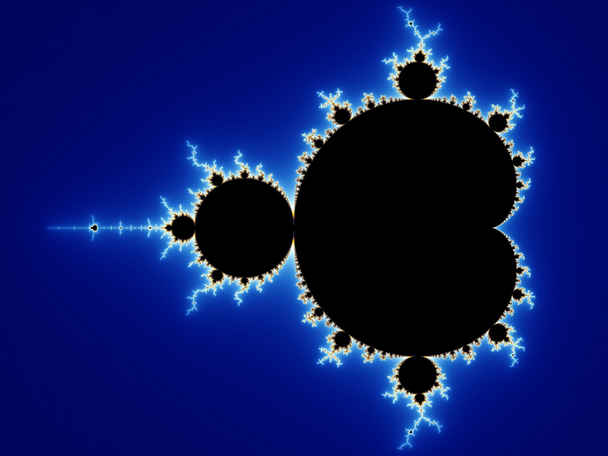
\includegraphics[width=0.85\textwidth]{papers/julia/imgs/mandelbrot2.png}

    \caption{Die Mandelbrot-Menge}
    \label{julia:fig:mandelbrot_definition}
\end{figure}

Anhand obiger Definition wird der grundliegende Unterschied zwischen Julia- und Fatou-Mengen sowie der Mandelbrot-Menge klar.
Die Julia- und Fatou-Mengen sind im Zustandsraum der Dynamik, sie sind Teilmengen der $z$-Ebene.
Bei der Mandelbrot-Menge findet die Dynamik zwar auch in der $z$-Ebene statt, jedoch existiert die Mandelbrot-Menge im Parameterraum bzw. der $c$-Ebene.

Die Mandelbrot-Menge liegt vollständig innerhalb eines Kreises mit Radius $2$, jedoch gehört nicht der gesamte Kreisinhalt zur Mandelbrot-Menge.
Möchte man untersuchen, ob ein bestimmter Parameter $c_i$ zur Mandelbrot-Menge gehört, ist $|z_n| < 2$ für alle $n$ eine \emph{notwendige}, jedoch \emph{nicht hinreichende} Bedingung.

\subsection{Aufbau der Mandelbrot-Menge}
Betrachtet man die Mandelbrot-Menge \ref{julia:fig:mandelbrot_definition} erneut, so wird klar dass diese aus mehreren Komponenten besteht.
In Verbindung mit der Überlegung, welche die Julia-Mengen motivierte, lässt sich so ein interessanter Umstand beobachten.

So gibt es zum Beispiel die sogenannte Kardioide, welche die herzförmige und grösste Region der Mandelbrot-Menge ist.
Für jeden Parameter $c$ in der Kardioide, besitzt die zugehörige Funktion $f_c$ einen \emph{anziehenden} Fixpunkt $z_0$ (siehe Abschnitt \ref{julia:arten_periodische_punkte}), so dass
\begin{equation*}
    f_c(z_0) = z_0
\end{equation*}
gilt.
Anstatt als Fixpunkt könnte man diesen Punkt auch periodisch, mit einer Periode von $1$ nennen.

Angrenzend an die Kardioide liegen mehrere kreisförmige Knospen, die grösste davon befindet sich links der Kardioide.
Innerhalb dieser Knospe gilt für jeden Parameter $c$, dass die zugehörige Funktion $f_c$ einen \emph{anziehenden} periodischen Punkt $z_0$ besitzt, von dem eine Folge mit Periode $2$ ausgeht.
Für jede dieser Funktionen gibt es also einen Startwert, von dem sich eine Folge
\begin{equation*}
    z_0 \mapsto z_1 \mapsto z_0 \mapsto z_1 \ldots
\end{equation*}
entwickelt.
Aufgrund der Periodizität bezeichnet man diese Region als Periode-2 Knospe.

Die kleineren kreisförmigen Knospen verhalten sich ähnlich, es gibt
\begin{itemize}
    \item Periode-3 Knospen,
    \item Periode-4 Knospen,
    \item und so weiter.
\end{itemize}
Man kann also jede Region der Mandelbrot-Menge mit einer Periode bezeichnen.
Die Kardioide besitzt die Periode $1$, die grösste kreisförmige Knospe eine Periode von $2$ und so weiter.
Die unterschiedlichen Regionen sind also nicht nur dekorativ, sondern korrespondieren zu unterschiedlichen Arten von nicht-chaotischem, periodischem Verhalten.

\subsection{Verallgemeinerungen}
Die Mandelbrot-Menge lässt sich auf verschiedene Arten verallgemeinern.
In diesem Abschnitt werden einige davon beschrieben.

\subsubsection{Multibrot-Mengen}
Multibrot-Mengen entstehen, wenn man statt einer quadratischen Funktion, Polynome eines beliebigen Grades betrachtet
\begin{equation*}
    f_c(z) = z^d + c.
\end{equation*}
Beispiele davon sind in Abbildung \ref{julia:fig:multibrot_mengen} dargestellt.
Dies kann weiter verallgemeinert werden, indem negative und rationale Zahlen als Exponent $d$ erlaubt werden.
\begin{figure}
    \centering
    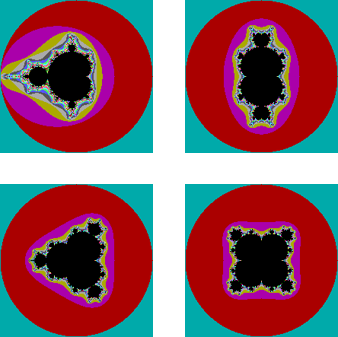
\includegraphics[width=\textwidth]{papers/julia/imgs/multibrot.png}

    \caption{Multibrot-Mengen für Polynome der Grade $2$, $3$, $4$ und $5$}
    \label{julia:fig:multibrot_mengen}
\end{figure}

\subsubsection{Höhere Dimensionen}
Statt den komplexen Zahlen kann auch mit \emph{Quaternionen} gearbeitet werden, diese sind die vierdimensionale Erweiterung der komplexen Zahlen.
Ein Quaternion wird als $q = a + bi + cj + dk$ notiert, mit $i^2 = j^2 = k^2 = ijk = -1$ und $i \ne j \ne k$.

Die vierdimensionale Mandelbrot-Menge kann dann in eine dreidimensionale Struktur projiziert werden, was jedoch relativ uninteressant ist, da es sich lediglich um die Mandelbrot-Menge, rotiert um die reelle Achse handelt \cite{julia:quaternionen}.

\subsubsection{Nicht-analytische Funktionen}
Statt holomorphen Funktionen können auch nicht-holomorphe bzw. nicht-analytische Funktionen verwendet werden.

Ein bekanntes Beispiel ist das Tricorn-Fraktal, dabei wird die Rekursion
\begin{equation*}
    z_{n+1} = \overline{z_n}^2 + c
\end{equation*}
verwendet.
Bevor $z_n$ quadriert wird, wird die komplexe Konjugation berechnet.

Ein weiteres Beispiel ist das Burning-Ship-Fraktal, welches durch die Rekursion
\begin{equation*}
    z_{n+1} = \left(|\text{Re}(z_n)| + i\,|\text{Im}(z_n)|\right)^2 + c
\end{equation*}
entsteht.
Anders als bei der Mandelbrot-Menge werden hier die Beträge des Real- und Imaginärteils berechnet, bevor quadriert wird.

\section{Beziehung Julia-Mengen und Mandelbrot-Menge}
\label{sec:relation}
% TODO
%% In Quelle julia:ähnlichkeit_mandelbrot zeigen Figure 1 (M) und Figure 2 (J) die Ähnlichkeit von Mandelbrot und Julia
%% https://en.wikipedia.org/wiki/Julia_set#Examples ist ein Beispiel wenn man Julia-Mengen nebeneinander legt, bekommt man irgendwann die Mandelbrot-Menge

\section{Visualisierung der Mengen}
\label{sec:visualisierung}
In den vorherigen Abschnitten wurden Bilder von der Mandelbrot-Menge sowie der Julia- und Fatou-Mengen gezeigt.
Nachfolgend wird beschrieben wie diese Mengen visualisiert werden.
Bei diesen Visualisierungen handelt es sich um \emph{Fraktale}, was bedeutet dass, unabhängig vom Vergrösserungsfaktor, stets neue Details und Strukturen erscheinen.
Diese Strukturen sind häufig selbstähnlich, heisst sie sind eingebettet in grössere Strukturen, die ähnlich aussehen.

\subsection{Visualisierung der Julia- und Fatou-Mengen}

\begin{aufgabe}
    Visualisierung Julia- und Fatou-Mengen
    \begin{enumerate}
        \item Funktion $f(z)$ wählen
        \item Die reelle und imaginäre Achse der $z$-Ebene plotten
        \item $f^n(z_i)$ für jeden Punkt $z_i$ dieses Koordinatensystems berechnen
        \item Punkte $z_i$ einfärben, je nachdem wie schnell und ob sie divergieren
    \end{enumerate}
\end{aufgabe}
Zu beachten ist, dass $n$ in der Theorie gegen unendlich geht, in der Praxis ist dies natürlich nicht möglich, je nach Rechenleistung muss ein genügend grosser Wert für $n$ gewählt werden.

Je nach gewählter Funktion und Farbschema können so sehr eindrückliche Bilder erstellt werden, wie zum Beispiel in Abbildung \ref{fig:bsp_julia}.
Interessant wird es besonders dann, wenn die Julia-Menge \emph{nicht zusammenhängend} ist (siehe Abschnitt \ref{sec:julia_connected}).
In diesem Fall besteht die Julia-Menge häufig nur aus einzelnen Punkten, während die übrigen Punkte zur Fatou-Menge gehören.

\begin{figure}
    \centering
    
\includegraphics[width=0.95\textwidth]{papers/julia/imgs/julia3.jpg}

    \caption{Beispiel einer Julia-Menge}
    \label{fig:bsp_julia}
\end{figure}

\subsection{Visualisierung der Mandelbrot-Menge}
\label{sec:visualisierung_mandel}

\begin{aufgabe}
    Visualisierung Mandelbrot-Menge
    \begin{enumerate}
        \item Beginne mit $f_c(z) = z^2 + c$
        \item Die reelle und imaginäre Achse der $c$-Ebene plotten
        \item $f^n_{c_i}(0)$ für jeden Punkt $c_i$ dieses Koordinatensystems berechnen
        \item Punkte $c_i$ einfärben, je nachdem wie schnell und ob sie divergieren
    \end{enumerate}
\end{aufgabe}
Der Ablauf ist im wesentlichen gleich wie bei den Julia- und Fatou-Mengen, der grosse Unterschied liegt darin, dass hier der Parameterraum bzw. die $c$-Ebene abgebildet wird.
Auch hier gilt in der Theorie $n \to \infty$, es muss wieder ein genügend grosser Wert für $n$ gewählt werden.

Je nach Farbschema führt auch dies zu sehr eindrücklichen Bildern, wie zum Beispiel Abbildung \ref{fig:bsp_mandelbrot}.

\begin{figure}
    \centering
    
\includegraphics[width=0.95\textwidth]{papers/julia/imgs/mandelbrot1.jpg}

    \caption{Beispiel der Mandelbrot-Menge}
    \label{fig:bsp_mandelbrot}
\end{figure}



\printbibliography[heading=subbibliography]
\end{refsection}
